
\label{sect:application}

Using the training algorithm described in Section \ref{sect:template_training}, we will learn galaxy SED templates directly from the broadband photometry described in Section \ref{sect:data}.
We divide the data set into a training and test set, consisting of random 80\% and 20\% samples respectively of the entire data set.
The training set will be used to train the SED templates, while the test set will be used to evaluate the learned templates via photo-z estimation (see Section \ref{sect:photoz}).
The training set consists of 81,980 galaxies, with mean redshift $z_\text{mean} = 0.69$, max redshift $z_\text{max} = 4.54$, and magnitudes $13.8 < i < 25.7$.
A full summary of the set can be seen in Table \ref{tab:data_sets}, and the redshift distribution can be seen in Figure \ref{fig:redshift_dist}.

Eight naive templates were chosen to represent the underlying SED shapes of the photometry set according to the principles described at the end of Section \ref{sect:training_sets}.
They are ``naive'' because they are simply chosen by eye to roughly divide the photometry into groups by spectral shape, but otherwise are not based on any theoretical models or observed SED's.
Each of the naive templates is a log-normal function,
\begin{align}
    S(\lambda) \propto \frac{1}{\lambda} \exp{\left[ -\frac{1}{2\eta^2} \left( \ln{\frac{\lambda}{\text{mode}(\lambda)}}-\eta^2 \right)^2 \right]},
\end{align}
normalized at $\lambda = 5000$ \AA, with $\text{mode}(\lambda)$ in the range $1000$ to $5500$ \AA\  and $\eta$ in the range $0.35$ to $0.9$. 
The templates extend to $15000$ \AA\ with 100 \AA\ resolution.
These eight templates (hereafter N8) can be seen together with with their original training sets in Figure \ref{fig:N8_untrained}.

\begin{figure*}
    \centering
    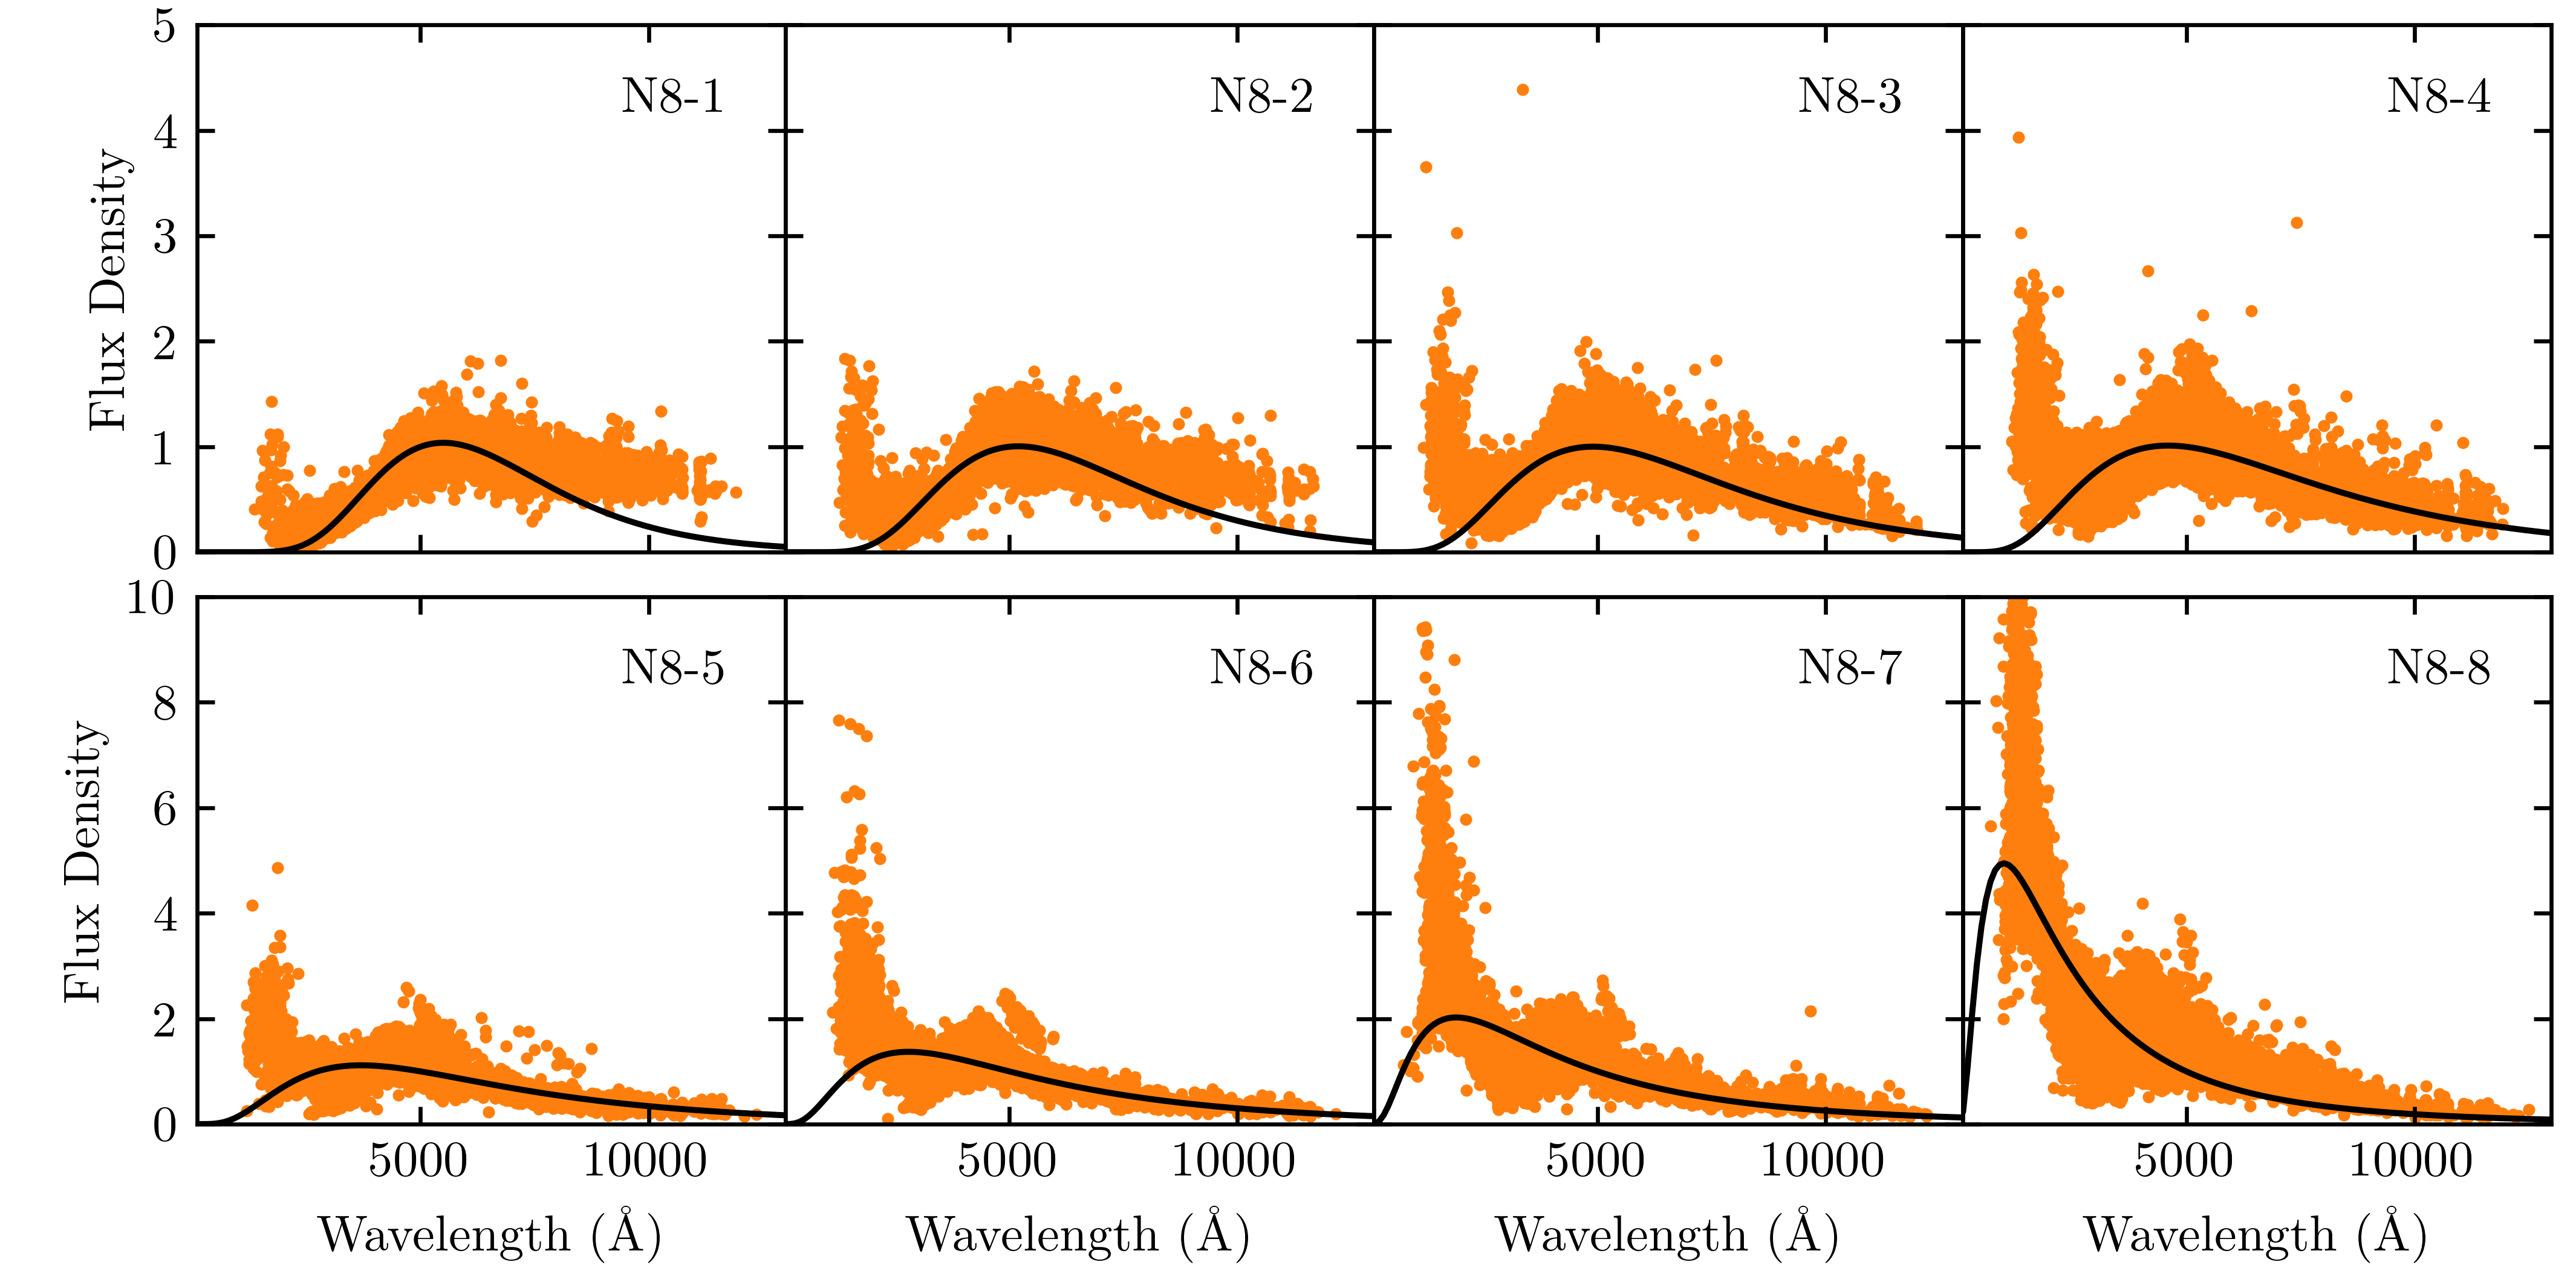
\includegraphics{figures/N8_untrained.png}
    \caption{The untrained N8 templates (black lines) with their corresponding photometry sets (orange points), generated with the algorithm described in Section \ref{sect:training_sets}. N8-1 is the reddest template, with each successive template getting bluer.}
    \label{fig:N8_untrained}
\end{figure*}

The training algorithm with $w=0.5$ is applied to the N8 templates.
The convergence of the templates is evaluated via the weighted mean square error,
\begin{align}
    \text{wMSE} = \sum_n \frac{1}{\sigma_n^2}(\hat{f}_n(\{\hat{s}_k\}) - f_n)^2.
\end{align}
Each template is perturbed until the change in wMSE is less than 3\%, which was chosen empirically to balance sufficient template reconstruction and the algorithm's runtime.
When every template has converged to its current photometry set, new photometry sets are generated.
Only those templates whose new photometry sets result in a greater than 3\% change in wMSE resume perturbation with their new sets.
This process is iterated until no template has a new photometry set that results in a greater than 3\% change in wMSE.
This indicates that the photometry is sorted into distinct sets, and that further perturbation is unlikely to improve the photometry-matching results.

The progress of the training algorithm is shown in Figure \ref{fig:training} for the template N8-1.
The left panel shows the progress of the perturbation algorithm as it deforms the originally smooth N8-1 template to better match the colors of the matched photometry sets.
In particular, N8-1 becomes redder and acquires higher resolution structure, which will be discussed below.
The middle panel shows the wMSE and the right panel shows the fractional change in the wMSE throughout the training.
Orange points indicate values after a photometry-matching stage, and blue points indicate values after a perturbation.
You can see that the wMSE drops as the template is perturbed, and perturbation continues until the magnitude of the fractional change in wMSE drops below 0.03, indicated by the dotted black lines in the right panel.
Once this occurs, new photometry is matched, resulting in an increase in wMSE.
This process is iterated, with fewer and fewer perturbations needed per iteration.
Eventually, all of the points are orange, indicating that after each new photometry matching, N8-1 is not perturbed, as it already sufficiently matches its photometry set.

\begin{figure*}
    \centering
    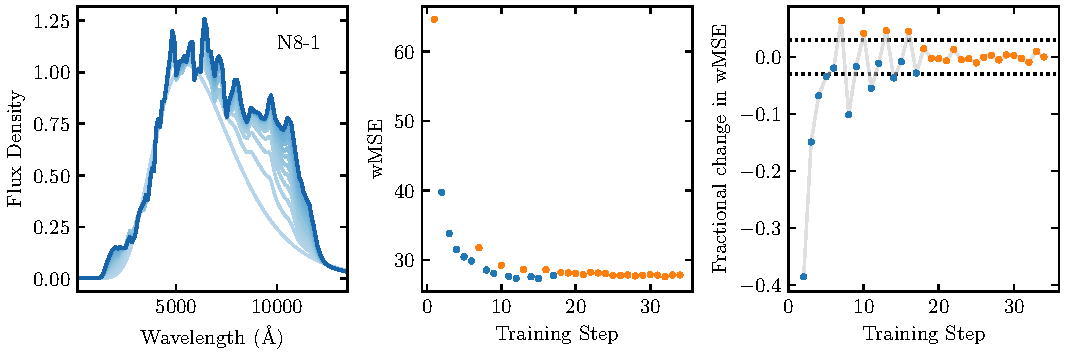
\includegraphics{figures/N8_1_training_history.pdf}
    \caption{Training of N8-1. Left: the initial (light blue) N8-1 template is iteratively perturbed to better represent the colors of its photometry set. The final (dark blue) template is redder and has more structure. Middle: wMSE of the N8-1 template throughout the training process. Orange points represent the wMSE after a photometry matching stage, while blue points represent the wMSE after a perturbation. Right: fractional change in the wMSE. Orange points represent the fractional change due to a new photometry matching stage, while blue points represent a fractional change due to a perturbation. The dotted black lines show the $\pm 0.03$ cutoff. When a perturbation results in a fractional change of magnitude less than 0.03, perturbation is halted and new photometry is matched. After the sixth photometry match, the template is not perturbed because it already sufficiently matches the photometry.}
    \label{fig:training}
\end{figure*}

The training continues for 12 rounds, and takes approximately 15 minutes.
The final results for the N8 templates can be seen in Figure \ref{fig:N8_trained}.
The templates are now a much better match to the photometry and more closely resemble physical galaxy spectra.
Most of the templates have a Balmer Break at 4000 \AA, although this was essentially already present in the initial templates.
In addition, there are now emission and absorption lines visible in the spectra at a much higher resolution than the broadband filters used for the photometry (some of which are labeled with gray lines in Figure \ref{fig:N8_trained}).
Template N8-1 displays Mg and Na absorption lines and template N8-4 contains the beginnings of $H\alpha$ and $H\beta$ emission lines.
Templates N8-6, N8-7, and N8-8 contain what appear to be H$\alpha$, H$\beta$, H$\gamma$, H$\delta$, OII, and OIII emission lines (see Section \ref{sect:speclines} for more analysis).
The emergence of these high resolution features from a large ensemble of low resolution data is the one of the defining features of this method.

\begin{figure*}
    \centering
    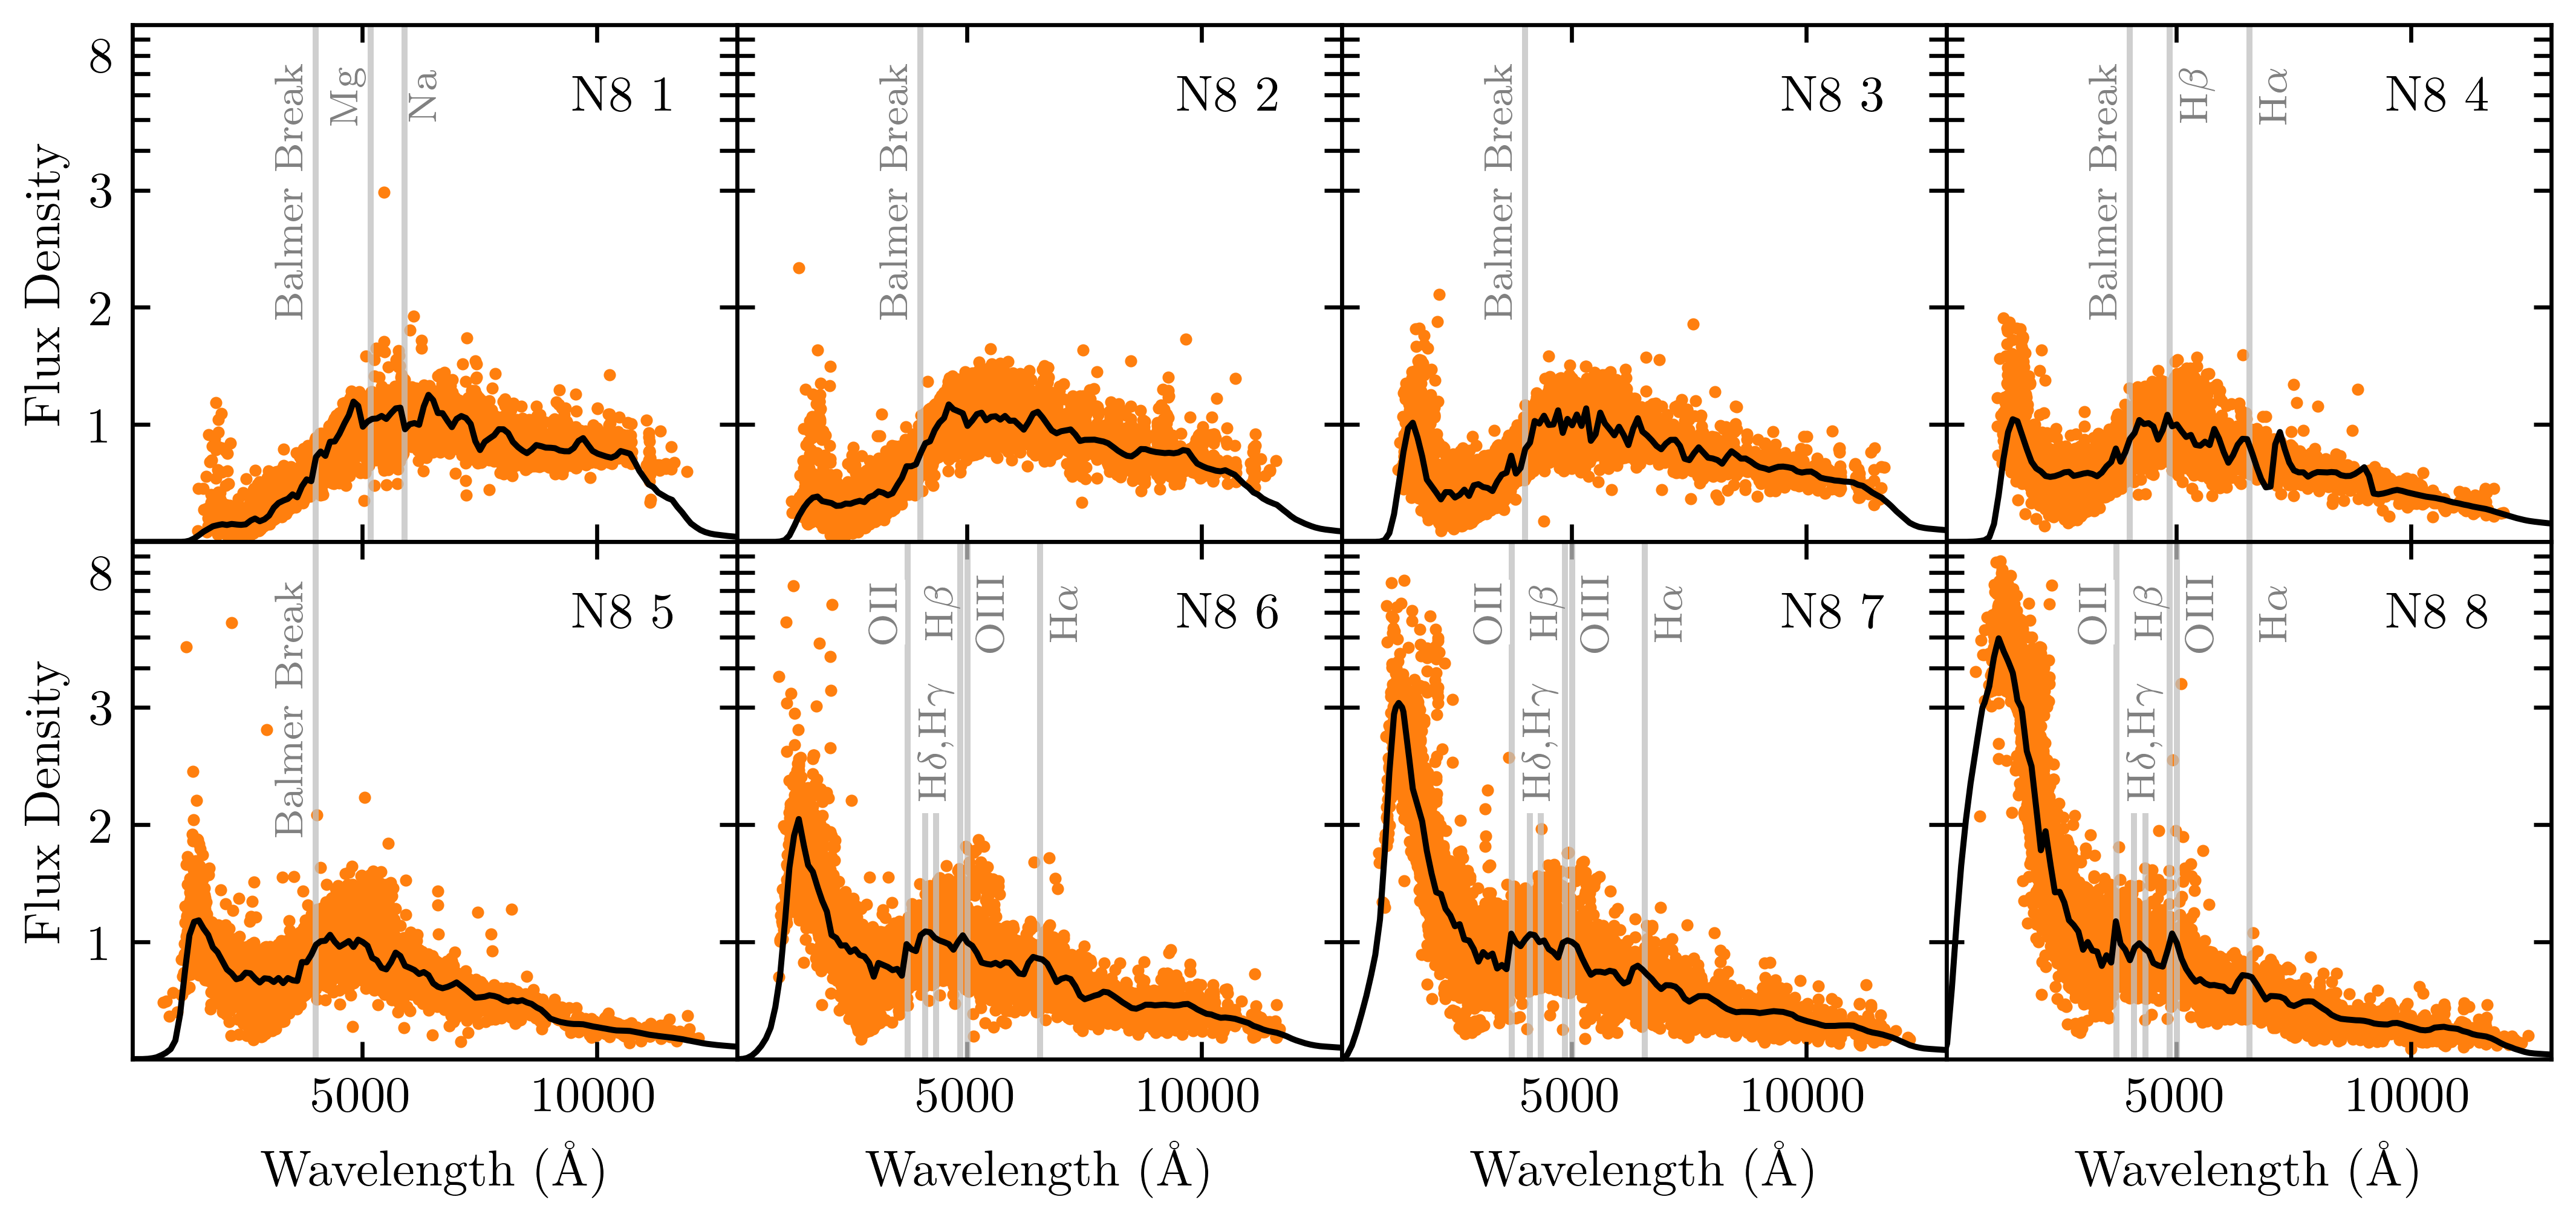
\includegraphics{figures/N8_trained.png}
    \caption{The trained N8 templates (black lines) with their final photometry sets (orange points). N8-1 is the reddest template, with each successive template getting bluer. The templates now more closely resemble physical galaxy spectra, and have acquired structure at a higher resolution than the broadband templates. The Balmer break, Mg and Na absorption lines, and H$\alpha$, H$\beta$, H$\gamma$, H$\delta$, OII, and OIII emission lines are labeled in gray.}
    \label{fig:N8_trained}
\end{figure*}

In addition to these eight templates, we also train a set of 16 templates from the same range of parameters for the log-normal distribution, creating a more gradual transition of the templates from red to blue. 
Training for this template set (hereafter N16) took 50 minutes over 26 rounds.
The results of the training can be seen in Figure \ref{fig:N16_trained}.
These results closely resemble the N8 results, with the same spectral features emerging.
However, the N16 set shows a more gradual transition from red to blue.

\begin{figure*}
    \centering
    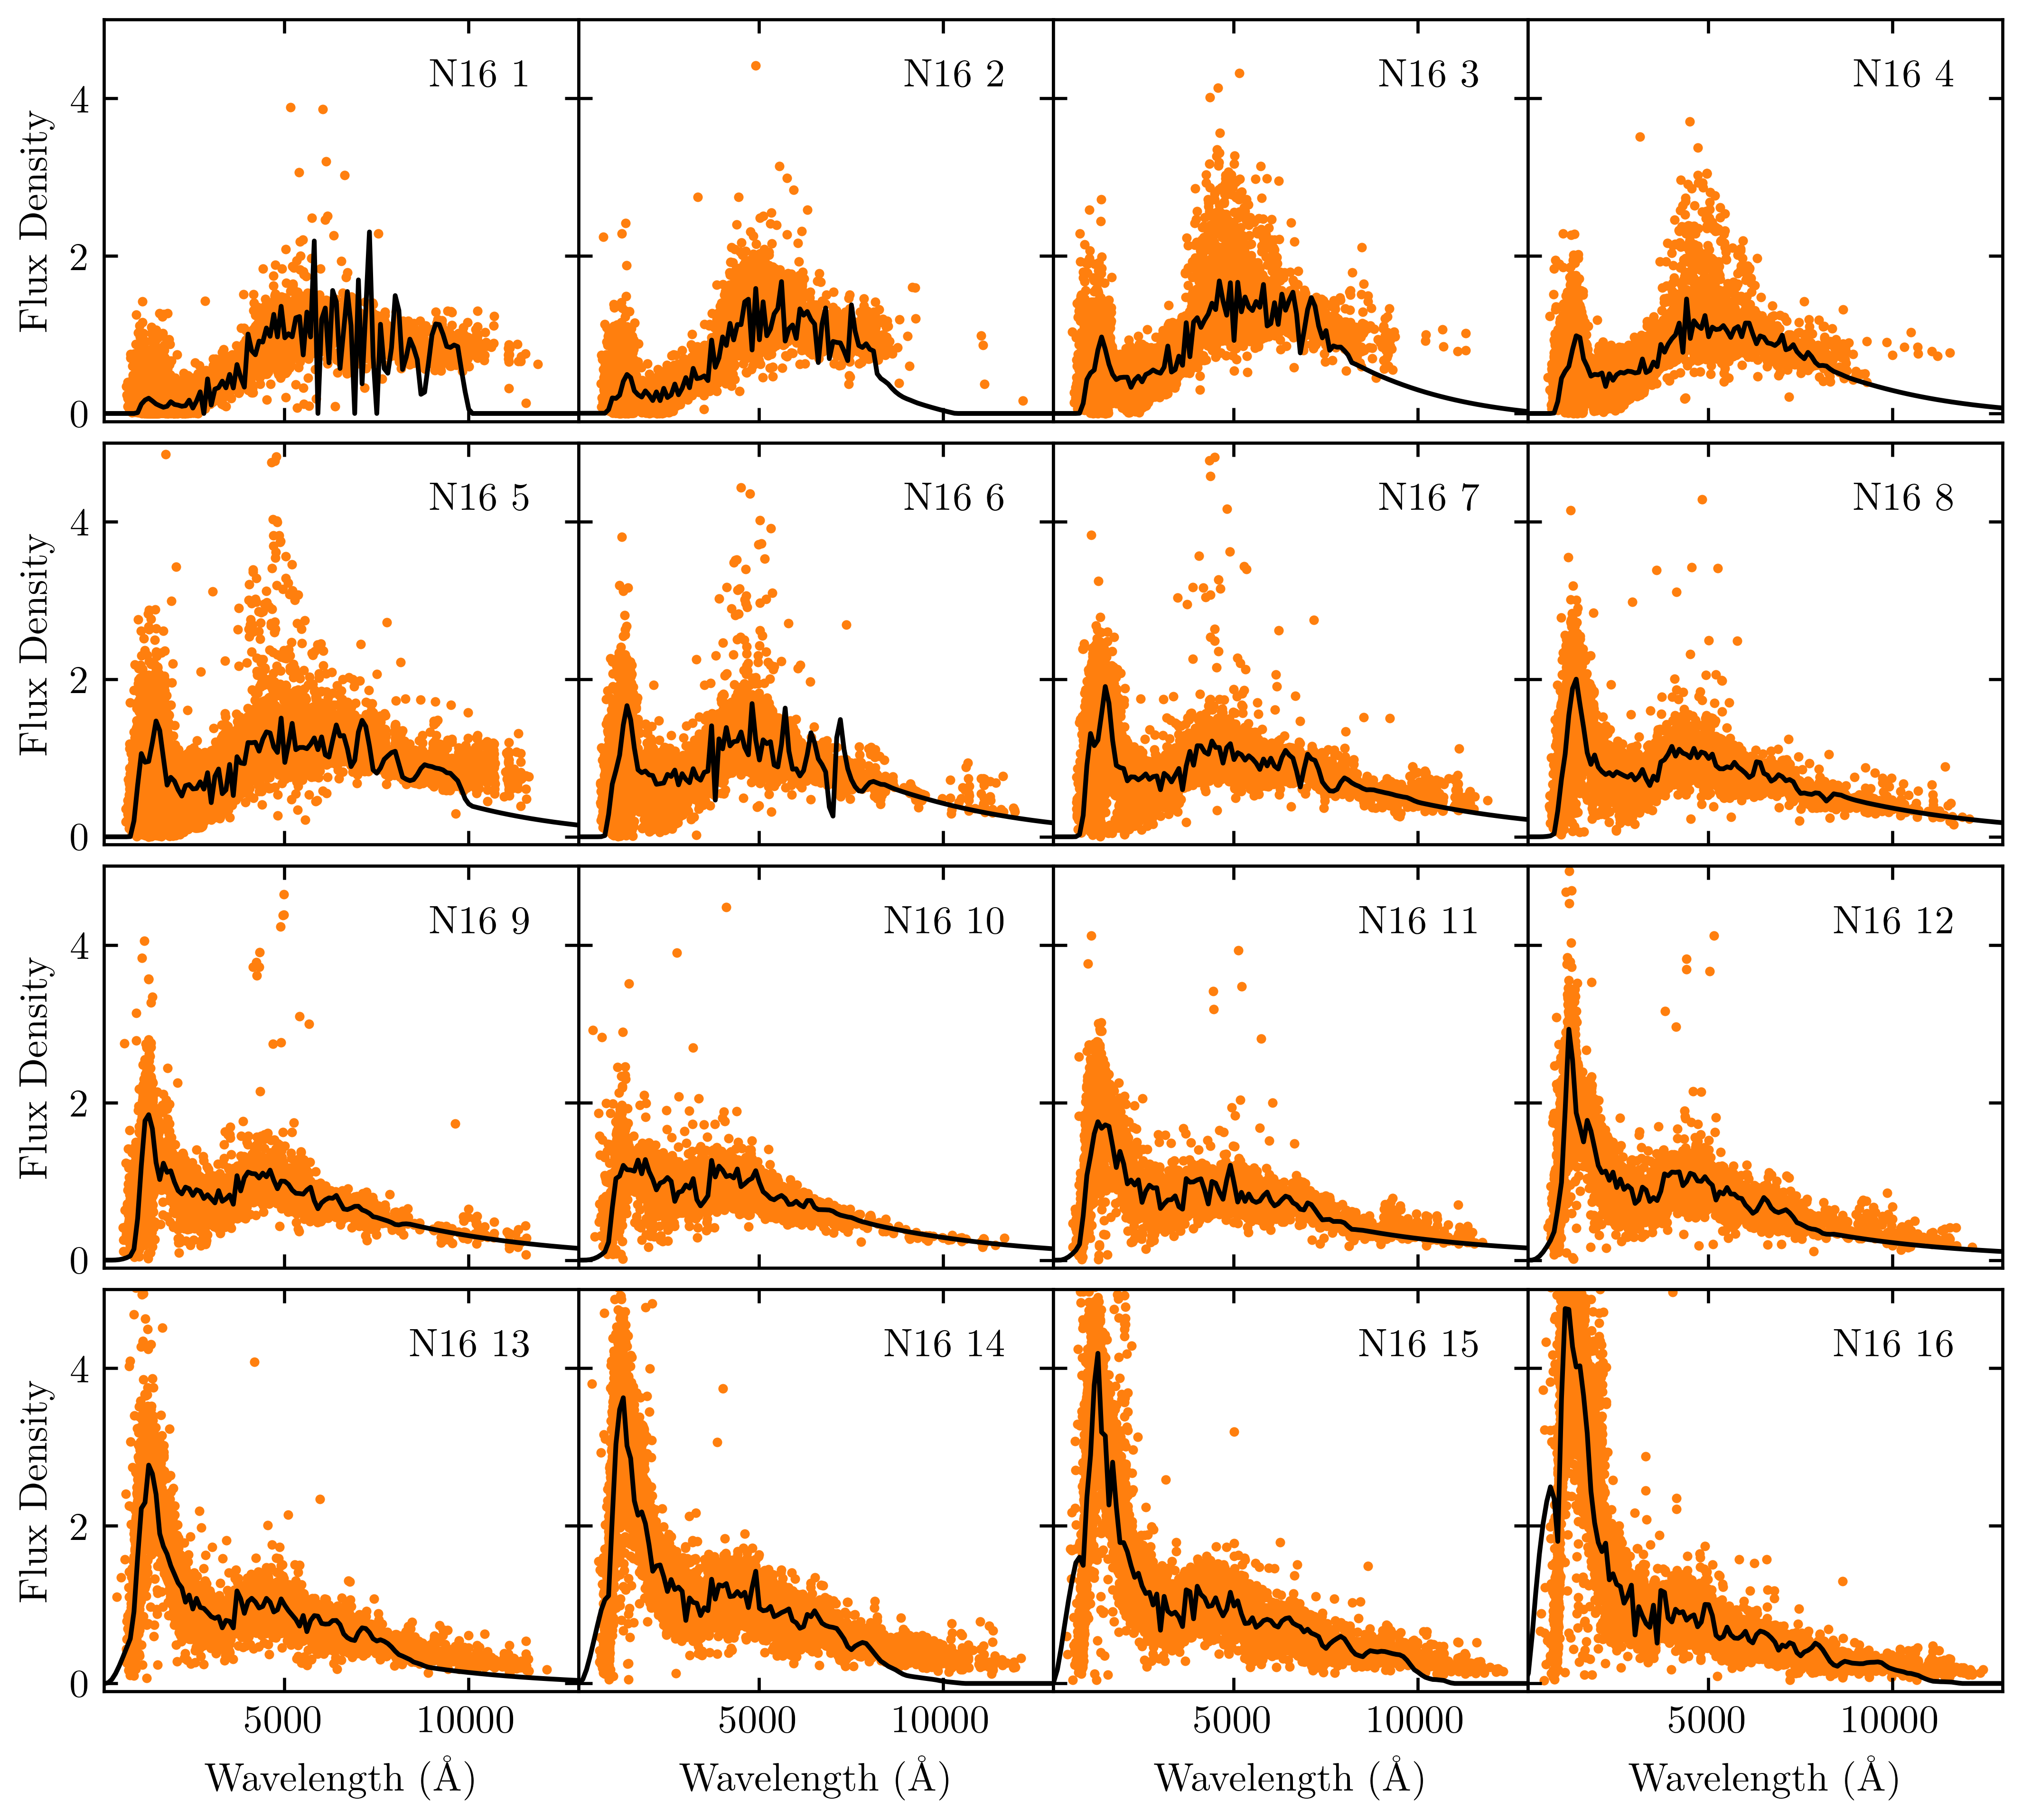
\includegraphics{figures/N16_trained.png}
    \caption{The trained N16 templates (black lines) with their final photometry sets (orange points). N16-1 is the reddest template, with each successive template getting bluer. These templates closely resemble the N8 templates and have show the same emerging spectral features (c.f. Figure \ref{fig:N8_trained}), but consist of a more continuous transition from red to blue spectra.}
    \label{fig:N16_trained}
\end{figure*}

In addition to starting from naive templates, one can start with templates derived from spectral synthesis models or observations of local galaxy spectra \citep{Budavari2000b, Csabai2000}.
Here we apply the training algorithm to a standard set of SED templates commonly used for photo-z estimation (e.g. \bpz, see Section \ref{sect:bpz}).
This set (hereafter CWW+SB4) consists of four templates from \citet{Coleman1980a} and two starburst templates from \citet{Kinney1996a}, the latter of which were added to account for faint blue galaxies in the HDF-N. 
These six templates were recalibrated by \citet{Benitez2004a} to correct for systematic differences between the observed and predicted galaxy colors in the HDF-N and other spectroscopic catalogs. 
In addition to these six, CWW+SB4 contains two synthetic starburst templates from \citet{Bruzual2003b}, added by \citet{Coe2006a} to account for even bluer galaxies in the UDF.

The CWW+SB4 templates were trained with $w=2$ for 46 minutes over 32 iterations.
The results of the training can be seen in Figure \ref{fig:cwwsb4_trained}.
The original templates are plotted in blue, with the trained templates plotted in black, along with the final photometry sets in orange.
You can see that the El and Sbc templates have barely been altered. The remaining templates have all systematically become redder.
The high resolution structure that was originally present in the Im, SB3, and SB2 templates have been decreased in magnitude, while additional structure has been added to the simulated 25Myr and 5Myr templates what were originally smooth.
These new features have been labeled in gray.

\begin{figure*}
    \centering
    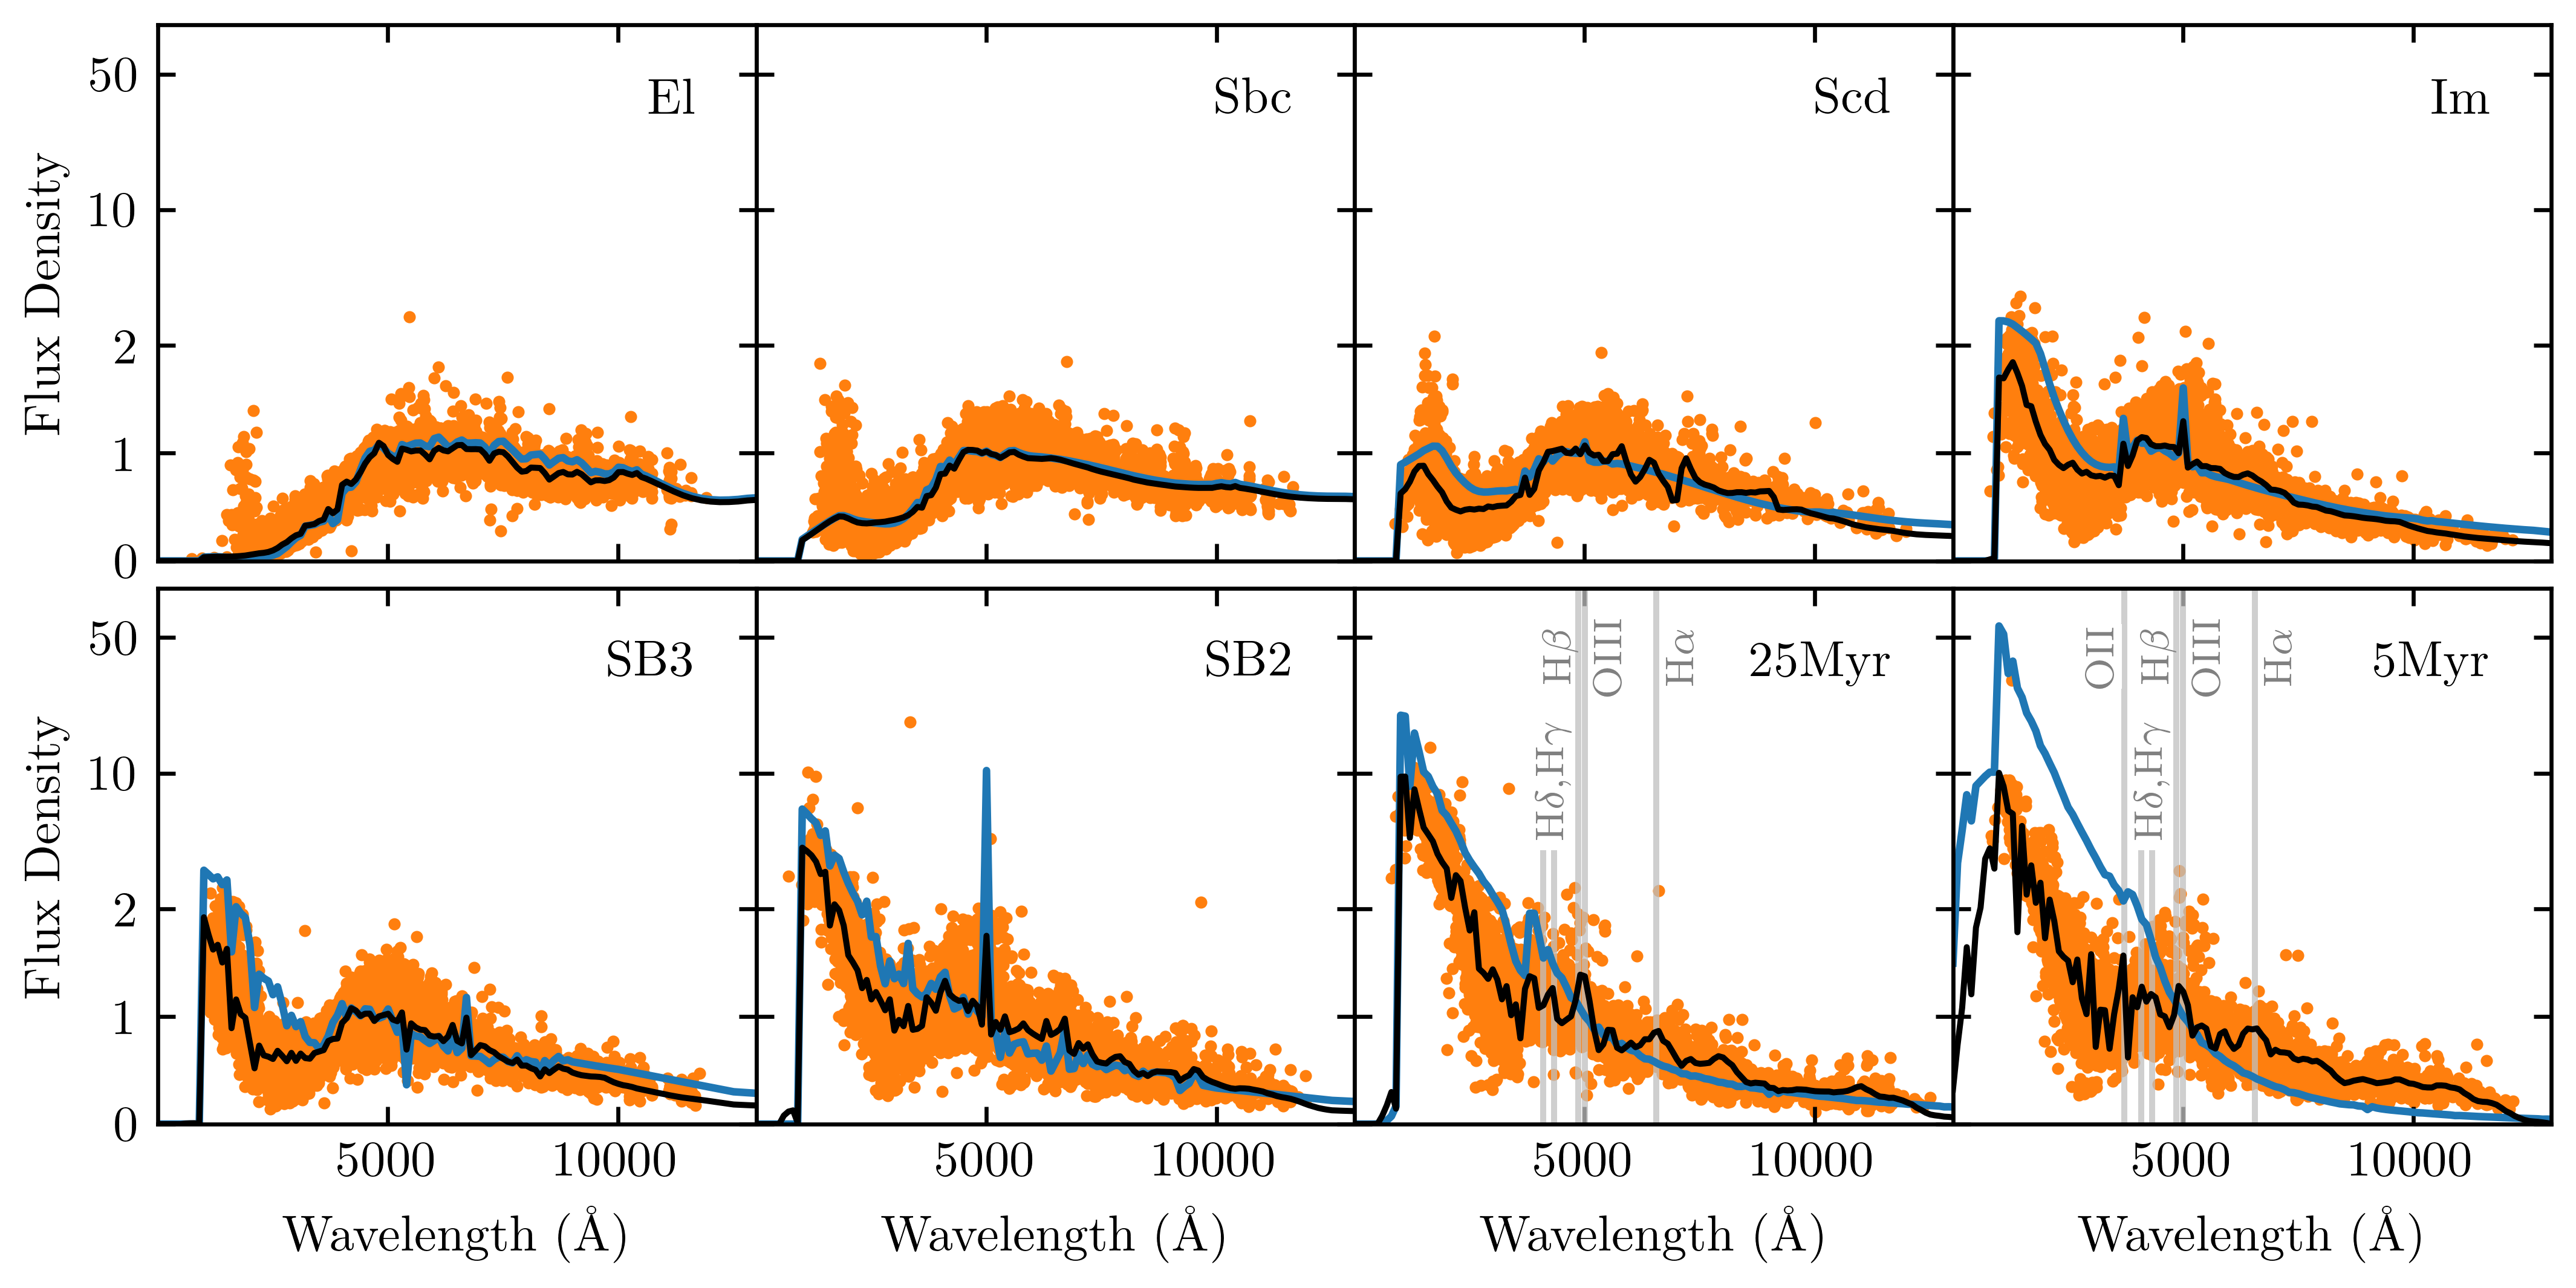
\includegraphics{figures/cwwsb4_trained.png}
    \caption{Result of training the CWW+SB4 templates. The original templates are in blue, the trained templates in black, and the final training sets are displayed as orange points. The 25Myr and 5Myr templates have acquired emission lines that were not present in the initial templates. These are labeled in gray.}
    \label{fig:cwwsb4_trained}
\end{figure*}



\subsection{Reconstructing Spectral Lines}
\label{sect:speclines}

The template training algorithm allows the reconstruction of high resolution spectral features from low resolution photometry due to the oversampling of the underlying SED templates.
This includes the emergence of spectral lines in many of the templates (c.f. Figures \ref{fig:N8_trained}, \ref{fig:N16_trained}, and \ref{fig:cwwsb4_trained}).
Knowledge of these lines allows us to perform post-processing of the learned templates to deconvolve the lines from the broadband filters.
Here we perform a simple post-processing of the N8-6, N8-7, and N8-8 templates to reconstruct the emission lines labeled in Figure \ref{fig:N8_trained}.
The templates are up-sampled to 10 \AA\ and the continuum of each is linearly interpolated around the emission lines.
The excess flux is attributed to the corresponding spectral lines. 
The flux of the H$\beta$ line is impossible to distinguish from the OIII line in our templates because they are so close to one another.
The same is true for the H$\gamma$ and H$\delta$ lines.
To overcome this difficulty, we use the Balmer decrements of $10^4$K SDSS galaxies from \citet{Groves2012a}: H$\alpha/$H$\beta = 2.86$ and H$\gamma/$H$\delta = 1.81$.
We calculate the H$\beta$ flux from H$\alpha$, and subtract this from the combined H$\beta$-OIII flux, and we calculate H$\gamma$ and H$\delta$ from the combined H$\gamma$-H$\delta$ flux.

After calculating the flux of the emission lines, the final templates are built by adding Gaussians of equivalent amplitude and FWHM = 20 \AA\ to the continuum. 
The templates with the reconstructed spectral lines can be seen in Figure \ref{fig:speclines}.
For each line, we calculate the amplitude relative to H$\beta$, and the effective width, $W_\lambda = \int (1 - F_\lambda/F_0) d\lambda$, where $F_\lambda$ is the total flux, and $F_0$ is the continuum flux.
These values can be seen in Table \ref{tab:speclines}.
Note that the amplitudes of our reconstructed H$\gamma$ and H$\delta$ lines relative to H$\beta$ are approximately three times greater than those listed in \citet{Groves2012a}.

\begin{table}
    \centering
    \caption{The emission lines reconstructed in the N8-6, N8-7, and N8-8 templates. For each line, we list the amplitude relative to H$\beta$, $r$, and the effective width, $W_\lambda$.}
    \begin{tabular}{c c | c r | c r | c r }
        \hline \hline
         & & \multicolumn{2}{c|}{N8-6} & \multicolumn{2}{c|}{N8-7} & \multicolumn{2}{c}{N8-8} \\
        \hline
         & $\lambda$ & $r$ & $W_\lambda$ & $r$ & $W_\lambda$ & $r$ & $W_\lambda$ \\
        \hline
        H$\alpha$ & 6563 & 2.86 & 132.7 & 2.86 & 103.3 & 2.86 & 115.2 \\
        H$\beta$  & 4861 & 1.00 &  32.9 & 1.00 &  26.4 & 1.00 &  30.3 \\
        H$\gamma$ & 4340 & 1.18 &  36.5 & 1.31 &  31.6 & 1.28 &  37.1 \\
        H$\delta$ & 4102 & 0.65 &  19.6 & 0.72 &  16.7 & 0.71 &  20.7 \\
        OII       & 3727 & 2.04 &  58.1 & 1.27 &  32.0 & 0.74 &  24.4 \\
        OIII      & 5007 & 2.08 &  68.0 & 2.42 &  66.1 & 0.86 &  27.3 \\

        \hline
    \end{tabular}
    \label{tab:speclines}
\end{table}

\begin{figure*}
    \centering
    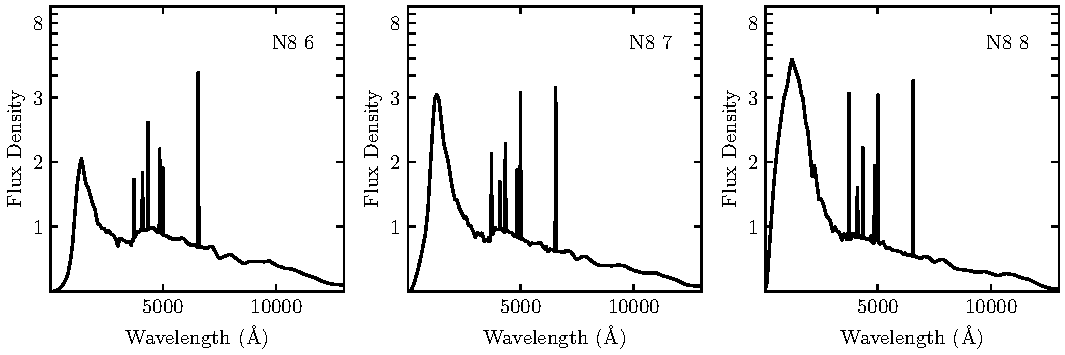
\includegraphics{figures/N8_spectral_lines.pdf}
    \caption{The N8-6, N8-7, and N8-8 templates with reconstructed emission lines (cf. Figure \ref{fig:N8_trained}). The emission lines, left to right, are OII,H$\delta$, H$\gamma$, H$\beta$, OIII, and H$\alpha$. The wavelengths, relative amplitudes, and effective widths of these lines are in Table \ref{tab:speclines}.}
    \label{fig:speclines}
\end{figure*}